\section{Evaluation of Environmental Wireless Sensor Networks (E-WSN)}
\label{section:experimental}	
\begin{figure}[ht]
	\centering
	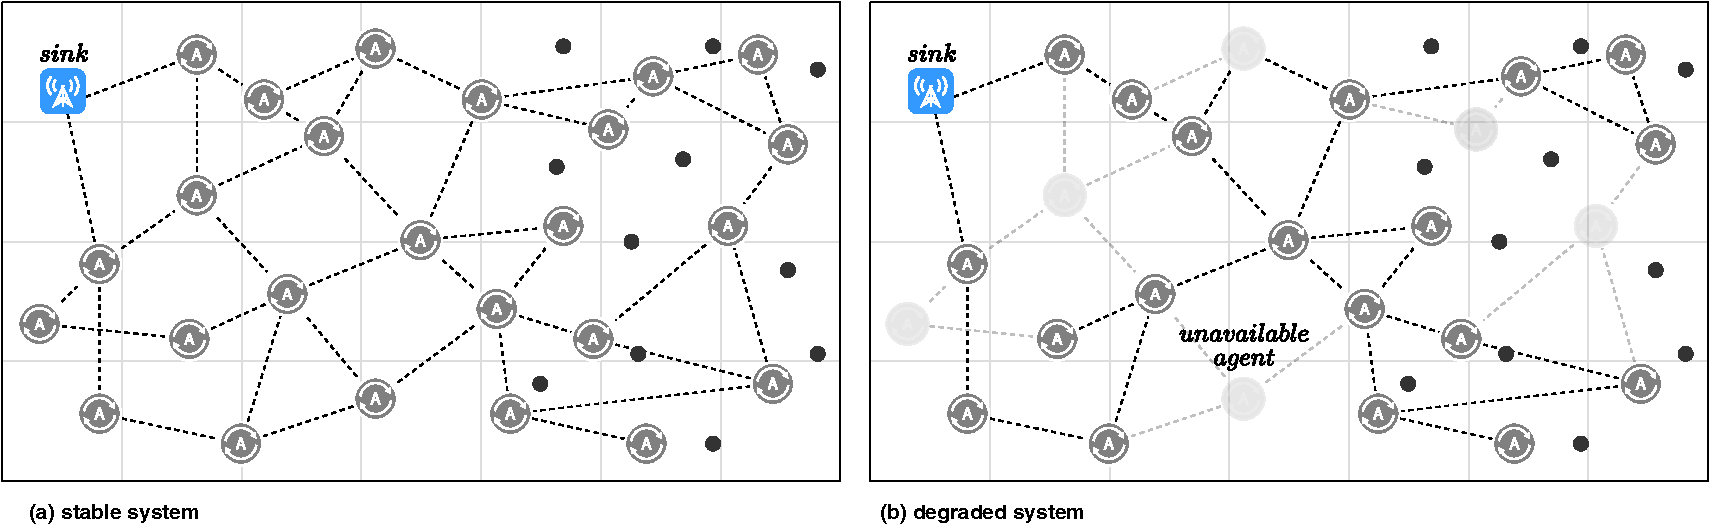
\includegraphics[width=0.9\linewidth, trim={25pt 0pt 25pt 0pt, clip}]{system-types}
	\caption{\textbf{System types}. The diagram shows examples of two systems. In the first, \simulationSimple{}{} system, there are $25$ agents that can execute the measurement tasks. The tasks' demand points are clustered away from the sink. In the second, \simulationNodeFailure{}{} system, a number of agents have failed, reducing the choice of task-paths, and so the possible optimisations.}
	\label{fig:system-types}
\end{figure}
\begin{figure}[ht]
	\centering
	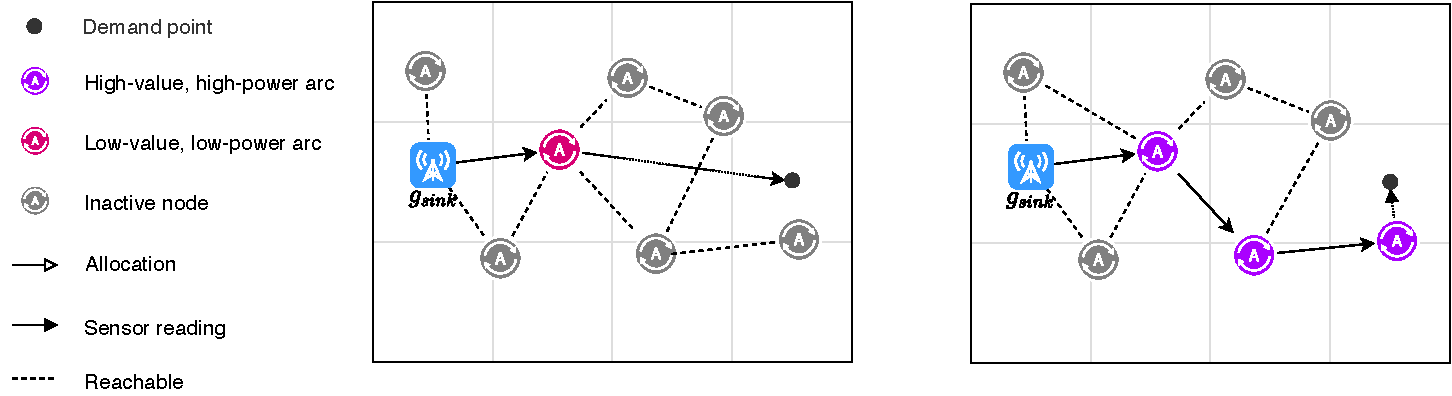
\includegraphics[width=0.9\linewidth, trim={25pt 0pt 25pt 0pt, clip}]{route-types}
	\caption{\textbf{Routes, power consumption, and task value}. The diagram shows two possible task-paths for the same system. In the first, energy is conserved by having a short task-path but the task is completed to a lesser quality. In the second, the maximum quality for the task is achieved, however, there is more energy consumption overall.}
	\label{fig:route_types}
\end{figure}

The simulation framework to evaluate the algorithms' performance was based on a realistic deployment scenario as covered by  \cite{Gomez2015} and others \citep{Jha2016, Avram}. In this scenario a UAV is used to deploy a large number of sensors over a expansive and remote geographical area, giving an ad-hoc, randomised placement of devices. Solar power cells are used to maintain enough energy to power the sensors over a number of years, given low enough power consumption. 

\subsection{Simulation types}
We ran $3$ simulations to evaluate the performance of the algorithm, using the \acronymQRouting{}{} algorithm \citep{Boyan} with a reward function based on the CTV from equation \ref{eq:taq} as a comparison. In the first simulation, the \simulationSimple{}{} system,  the \acronymWSNOptimisation{}{} algorithm had
equal weighting for each of the CTV components $\alpha, \beta, \gamma$ (Eq. \ref{eq:taq}) to examine system utility and energy optimisation in comparison to \acronymQRouting{}{}.  We then looked at the same configuration in the \simulationExtended{}{} system but where the energy, quality, and distribution CTV components were each given an $80\%$ dominance over the other components in $3$ separate configurations of the algorithm (Table \ref{table:summary_of_configurations}). By evaluating the algorithm in different configurations we could see how adaptable it was to different system goals such as being more quality, energy-efficiency, or distribution focused. Finally we looked at the \simulationNodeFailure{}{} system which had the addition of simulated system degradation through node failures. This studied how this instability effected optimisation and task-coverage.  

In the all systems there was  $1$ sink node and $25$ other agents distributed randomly. Each was initially connected to $3$ other agents that were randomly chosen with a bias towards nearby agents\footnote{
		The probability of initial agent selection used the standard gamma distribution $f(x; \alpha, \beta) = \frac{\beta^{\alpha} x^{\alpha-1}e^{- \beta x}}   {\Gamma(\alpha)}$, where $\Gamma(\alpha)$ is the  gamma function, $\alpha=1.8, \beta=0.5$, and $x$ is the unit distance between the two agents.
	}. 
The sink node was given $3$ composite tasks to complete sequentially, each consisting of $10$ different atomic measurement tasks. The demand points of the atomic tasks were configured to be distributed further away from the sink node rather than randomly distributed. The completion of the $3$ composite tasks marked the end of an episode, and the process was repeated for $1000$ episodes. Each non-sink node was capable of completing an atomic task, or allocating it to any of $3$ agents it was connected to. They could complete any measurement task with a quality dependent on their closeness to the demand point associated with the task (Eq. \ref{eq:atomic_task_quality}). The energy of all agents in the system was fully reset at the end of each episode. An example of this system layout can be seen in Figure \ref{fig:system-types}. 

The \simulationNodeFailure{}{} system introduced random node failures to the system over time, showing how each algorithm maintains coverage and optimises for quality and energy while some node availability is lost. The simulation ran for $100$ episodes, where for each episode between $20$ and $40$  a randomly chosen single node might fail with probability $0.25$. Once a node failed, it was unresponsive for all further episodes. 

 
